\documentclass{article}
\usepackage[margin=1in]{geometry}
\usepackage{amsmath}
\usepackage{listings}
\usepackage{color}
\usepackage{graphicx}
\usepackage{subfig}
\usepackage{blkarray}
\usepackage{multirow}
\usepackage{float}


\definecolor{dkgreen}{rgb}{0,0.6,0}
\definecolor{gray}{rgb}{0.5,0.5,0.5}
\definecolor{mauve}{rgb}{0.58,0,0.82}

\lstset{frame=tb,
  language=Python,
  aboveskip=3mm,
  belowskip=3mm,
  showstringspaces=false,
  columns=flexible,
  basicstyle={\small\ttfamily},
  numbers=none,
  numberstyle=\tiny\color{gray},
  keywordstyle=\color{blue},
  commentstyle=\color{dkgreen},
  stringstyle=\color{mauve},
  breaklines=true,
  breakatwhitespace=true,
  tabsize=3
}

\begin{document}
\begin{titlepage}
	\setlength{\parindent}{0pt}
	\large

\vspace*{-2cm}


University of Waterloo \par
CS 480 \par
\vspace{0.05cm}
r2knowle: 2023-09-20
\vspace{0.2cm}

{\huge Exercise \# 4 \par}
\hrule

\vspace{0.5cm}
\textbf{Q1)} Below is the implementation of KNN done in python which runs in O(nd) time:
\begin{lstlisting}
def partition(arr, low, high): 
    pivot = arr[high]
    i = low - 1
    for j in range(low, high):
        if arr[j] <= pivot:
            arr[i + 1], arr[j] = arr[j], arr[i + 1]
            i += 1

    arr[i + 1], arr[high] = arr[high], arr[i + 1]
    return i + 1

def quickselect(arr, low, high, k):
    if low < high:
        pivot_index = partition(arr, low, high)
        if pivot_index == k:
            return
        elif pivot_index < k:
            quickselect(arr, pivot_index + 1, high, k) 
        else:
            quickselect(arr, low, pivot_index - 1, k)


def KNN (X, Y, x_target, k):
    solutions = []
    for idx in range(0, len(X)): # ND time complexity
        distance = np.linalg.norm(X.iloc[idx] - x_target)
        y_label = pd.to_numeric(Y.iloc[idx,0])
        solutions.append((distance, y_label))
    quickselect(solutions, 0, len(solutions)-1, k-1) # ND time complexity
    solutions = solutions[0:k] # K time complexity
    sum = 0
    for tuple in solutions: # K time complexity
        sum += tuple[1]
    average = sum / k

    return average
\end{lstlisting}
Our algorithm has 4 main steps that it uses to calculate KNN. The first step is to calculate the distance of each point to the target point, this is done in O(nd) time as we look through the n points d dimensions. The next step is to select the k smallest distances, using quick sort and a pivot on average this will only take O(n) time, this is because the array we are sorting becomes smaller and smaller (as we cut it depending on the pivot) and we only need to sort a subset of it. Lastly the two steps of taking the k elements and finding the average of the k elements take O(K) time. Thus our total time complexity is:
\[ \text{time complexity: } O(nd + n + k + k) \]
However since $k<n$, and since $d>1$ we also have that $nd > n$. it thus follows that nd will dominate our other time complexity and our total time complexity is:
\[ \text{time complexity: } O(nd) \]
\newpage
\textbf{Q2)} Below are the requested graphs for dataset D, on the left shows the predictions of KNN and LSLR. On the right shows the means squared error: \\

\begin{figure}[H]
    \centering
{{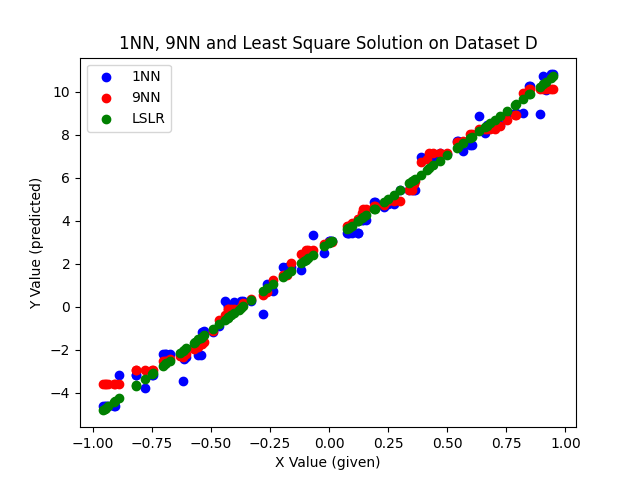
\includegraphics[width=7cm]{D_1.png} }}%
    \qquad
{{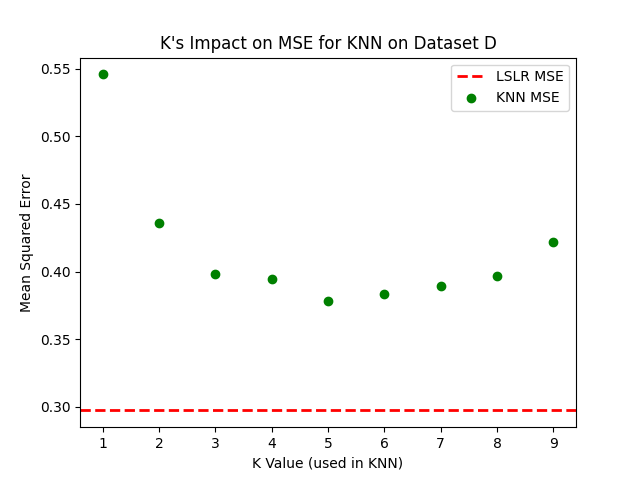
\includegraphics[width=7cm]{D_2.png} }}%
\end{figure}


Note that since the data seems to be generated from a linear distribution that the least square solution always out preforms the KNN. This is because our least square linear regression will minimize the half space for a linear distribution, so KNN could only at the very best on such a distribution do as good or worse. Therefore in this case least square linear regression does better on dataset D then KNN. \\

Next we will look at dataset E, on the left shows the predictions of KNN and LSLR. On the right shows the means squared error: \\

\begin{figure}[H]
    \centering
{{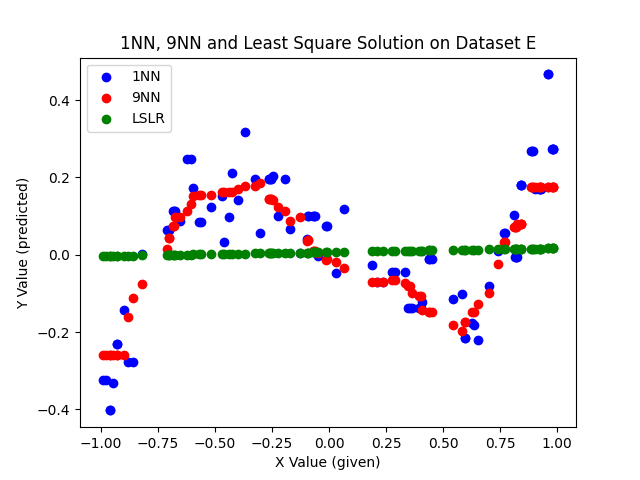
\includegraphics[width=7cm]{E_1.png} }}%
    \qquad
{{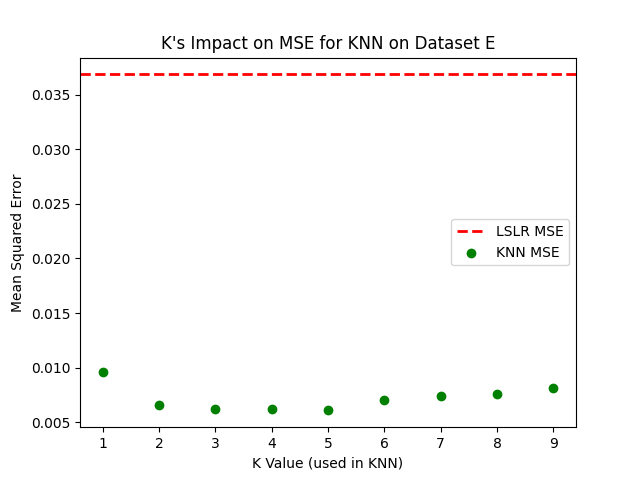
\includegraphics[width=7cm]{E_2.png} }}%
\end{figure}


From the graphs its evident that the data seems to follow a quadratic pattern, because of this LSR fails greatly and has a very large MSE. On the other hand KNN does exceptionally well and classifies the points well for many value so of k. However, this important to note that as k increase our MSE will increase as well, so it might not be the case that all for all values of k KNN will out preform LSLR. However for any k between 1 and 9 we can say for certain that KNN fits the data and produces less error then LSLR on dataset E.
\newpage
Below is the graph showing the MSE for different values of KNN and a horizontal line showing the MSE of LSLR:

\begin{center}
\textbf{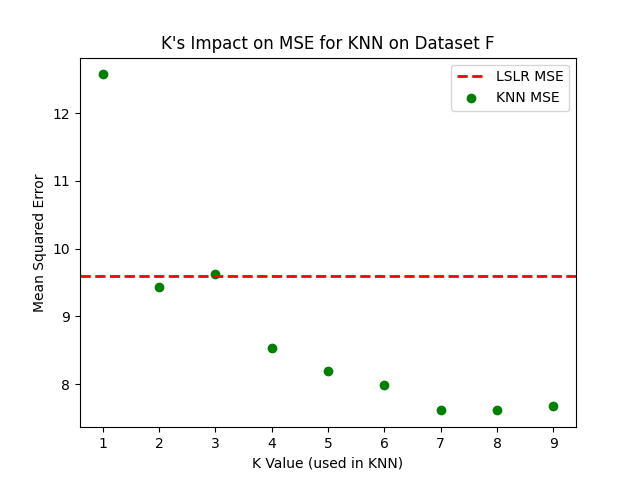
\includegraphics[width=14cm]{F_1.png}}
\end{center}

From this we can see that both strategies are very poor at predicting values with such high dimensionality, this is partly due to the fact that our training data is very limited and we have a large number of "features" or dimensions that we need to determine. There's also a very large distance between each of the points as the euclidean distance is greatly impacted by an increased dimensionality which impacts the accuracy of our predictions. In conclusion however it would appear that some value of KNN (like k=4,5,6) seem to out preform the LSLR for dataset F.
\end{titlepage}
\end{document}